% Created 2019-07-16 mar 13:49
\documentclass[presentation,aspectratio=169]{beamer}
\usepackage[utf8]{inputenc}
\usepackage[T1]{fontenc}
\usepackage{fixltx2e}
\usepackage{graphicx}
\usepackage{longtable}
\usepackage{float}
\usepackage{wrapfig}
\usepackage{rotating}
\usepackage[normalem]{ulem}
\usepackage{amsmath}
\usepackage{textcomp}
\usepackage{marvosym}
\usepackage{wasysym}
\usepackage{amssymb}
\usepackage{hyperref}
\tolerance=1000
\usepackage{khpreamble}
\usepackage{amssymb}
\usetheme{default}
\author{Kjartan Halvorsen}
\date{2018-08-08}
\title{Computerized control - Introduction}
\hypersetup{
  pdfkeywords={},
  pdfsubject={},
  pdfcreator={Emacs 24.5.1 (Org mode 8.2.10)}}
\begin{document}

\maketitle


\section{Intro}
\label{sec-1}
\begin{frame}[label=sec-1-1]{Feedback control}
\begin{center}
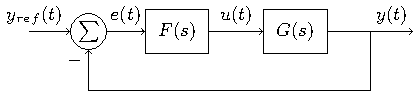
\includegraphics[width=0.6\linewidth]{../figures/block1}
\end{center}
\end{frame}
\begin{frame}[label=sec-1-2]{Feedback control}
\begin{center}
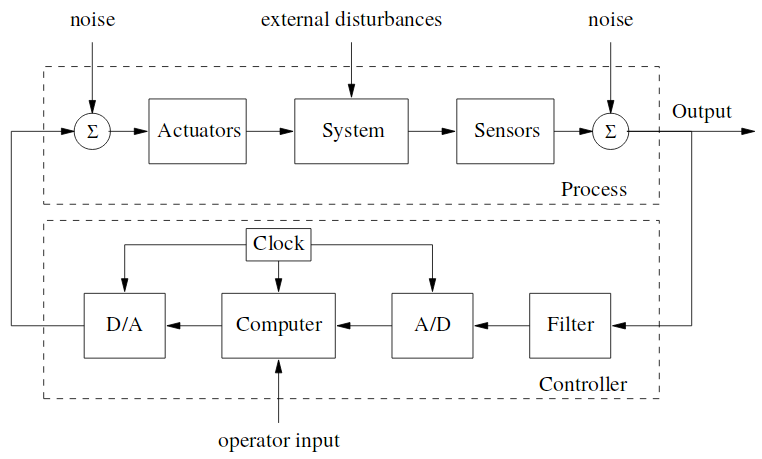
\includegraphics[width=0.7\linewidth]{../figures/comp-contr-sys.png}
\end{center}
\end{frame}

\begin{frame}[label=sec-1-3]{Why computerized control?}
\end{frame}

\begin{frame}[label=sec-1-4]{Computers everywhere}
\begin{center}
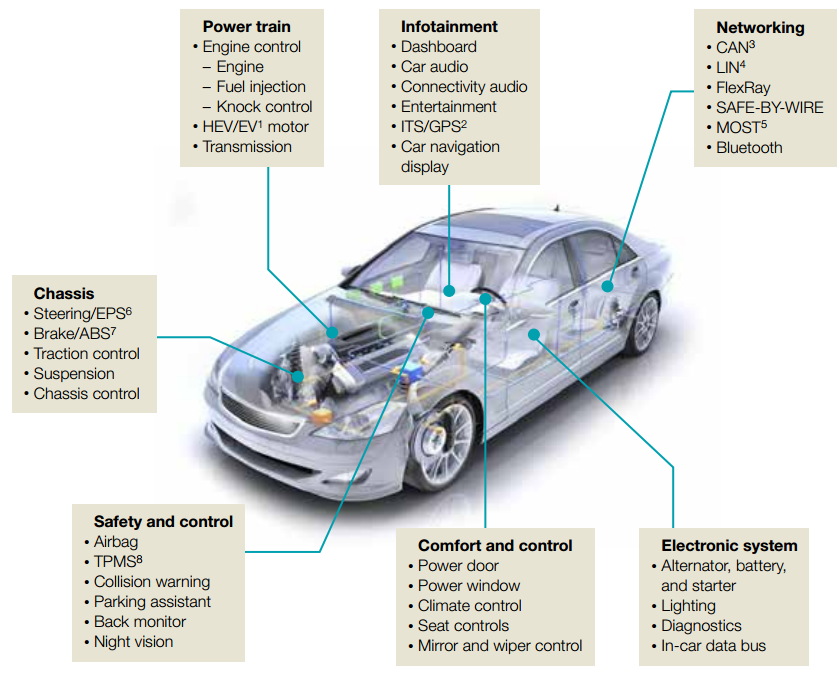
\includegraphics[width=0.7\linewidth]{../figures/electronics-in-cars.png}
\end{center}
{\tiny Winning share in automotive semiconductors. McKinsey report 2013 } 
\end{frame}

\begin{frame}[label=sec-1-5]{Discrete design can give better performance}
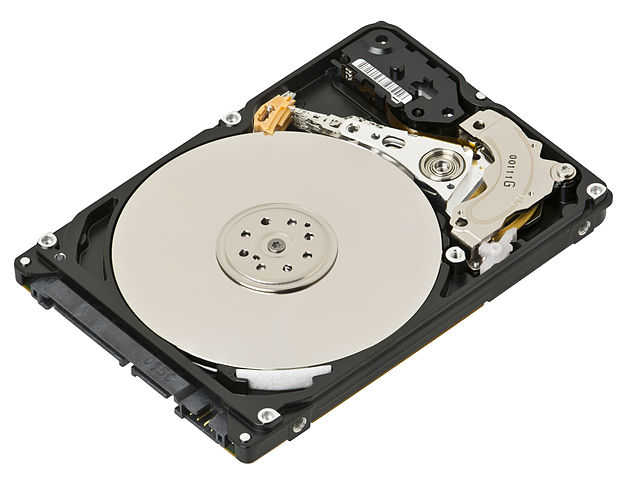
\includegraphics[height=0.5\textheight]{../figures/diskdrive.png}
\end{frame}

\begin{frame}[label=sec-1-6]{Discrete design can give better performance}
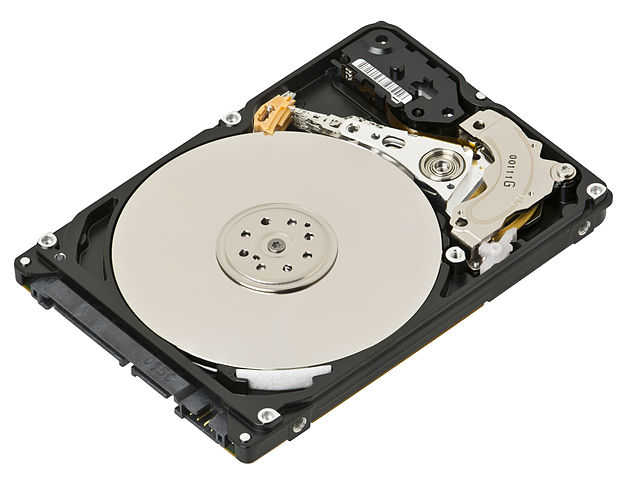
\includegraphics[height=0.5\textheight]{../figures/diskdrive.png}
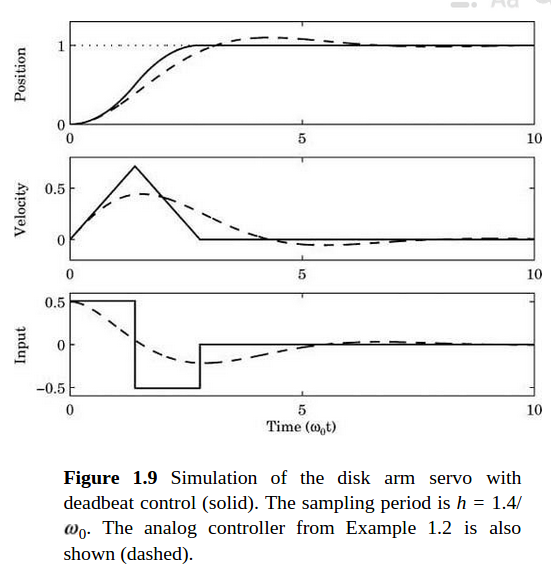
\includegraphics[height=0.8\textheight]{../figures/fig1-9.png}
\end{frame}

\begin{frame}[label=sec-1-7]{Why computerized control?}
\begin{itemize}
\item Almost all control systems are implemented on computers/microcontrollers
\item Controllers designed in continuous-time must be discretized to be implemented on a computer - What does this mean for the performance?
\item Design that takes into account the discrete nature of the computer can give better performance
\end{itemize}
\end{frame}

\begin{frame}[label=sec-1-8]{Challenges with computerized control}
\begin{block}{Aliasing}
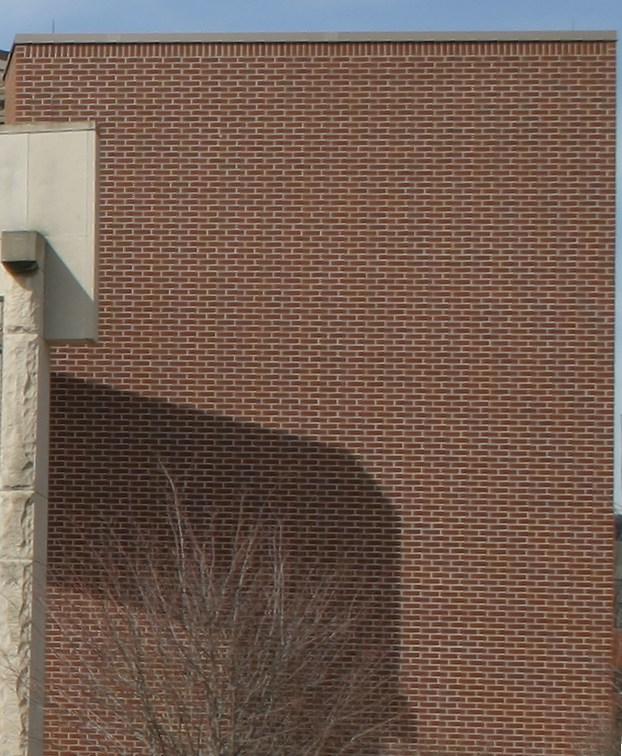
\includegraphics[height=0.6\textheight]{../figures/Moire_pattern_of_bricks.png} \hspace*{3mm} 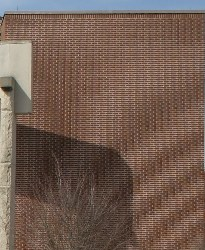
\includegraphics[height=0.6\textheight]{../figures/Moire_pattern_of_bricks_small.png}
\end{block}
\end{frame}

\begin{frame}[label=sec-1-9]{Challenges with computerized control}
\begin{block}{Sampling causes delay}
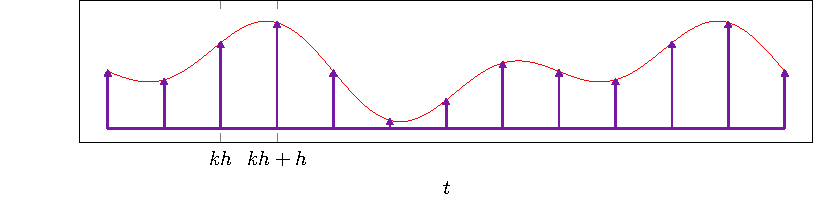
\includegraphics[width=0.9\textwidth]{../figures/modulation-model-timeseries}
\end{block}
\end{frame}


\begin{frame}[label=sec-1-10]{Goal of the course}
To be able to \alert{analyze}, \alert{design} and \alert{implement} an appropriate discrete-time controller to meet given performance criteria.
\end{frame}

\section{Presentation}
\label{sec-2}
\begin{frame}[label=sec-2-1]{Who am I?}
\begin{center}
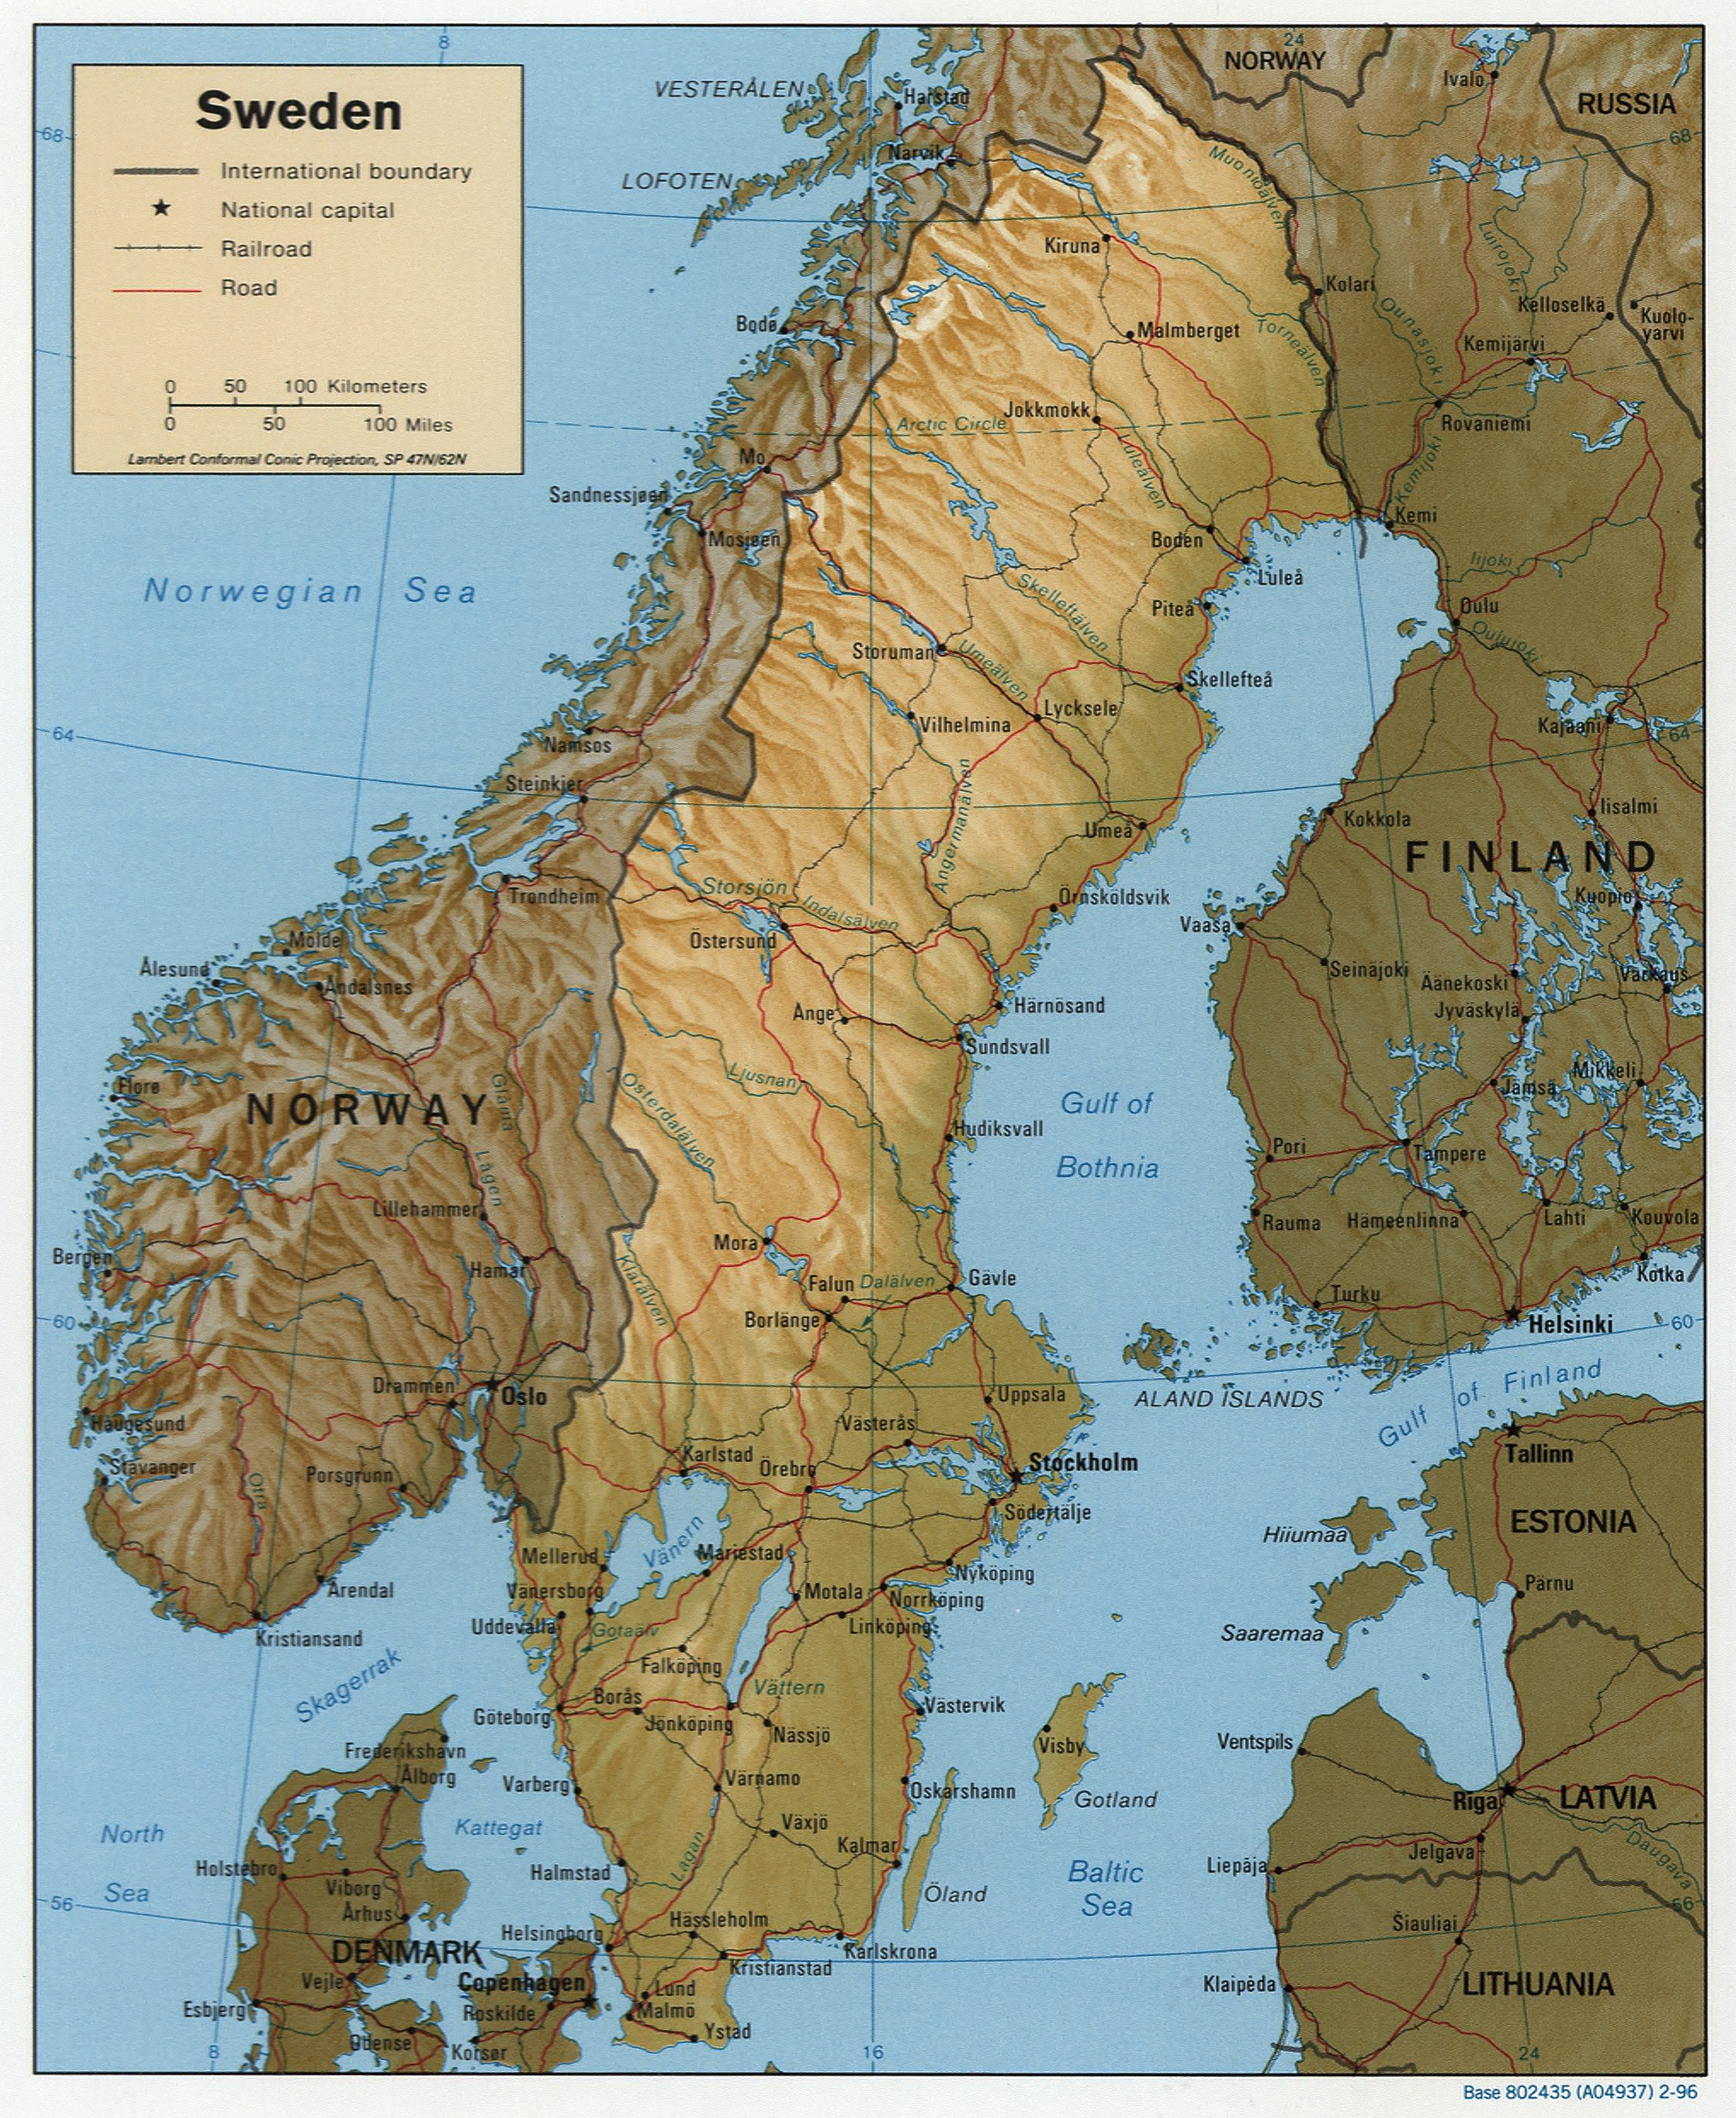
\includegraphics[width=0.4\linewidth]{../../MR2004/figures/map.png}\\
\end{center}
\end{frame}

\section{Who are you}
\label{sec-3}
\begin{frame}[label=sec-3-1]{Who are you?}
\end{frame}

\section{Course content structure}
\label{sec-4}

\begin{frame}[label=sec-4-1]{Control concepts}
\begin{center}
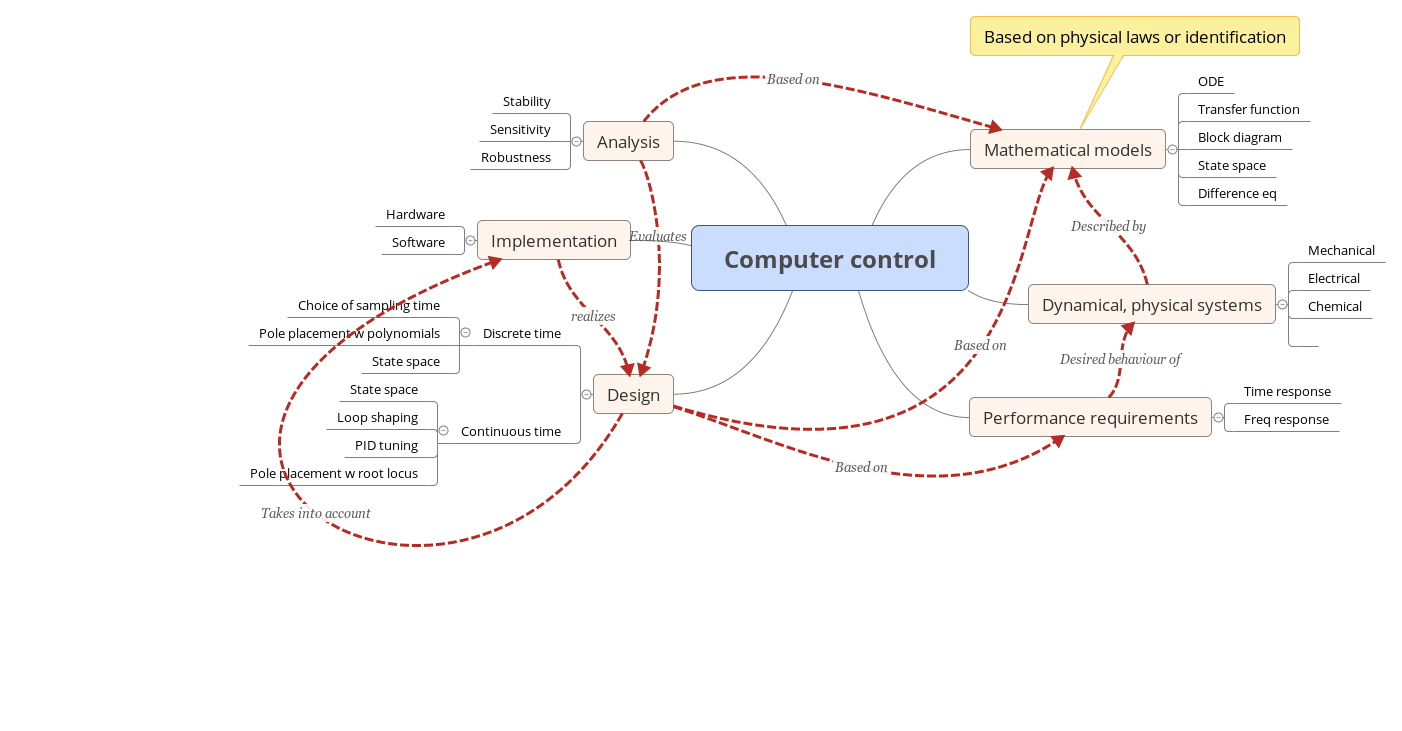
\includegraphics[width=1.1\linewidth]{../figures/computercontrol.png}
\end{center}
\end{frame}
\begin{frame}[label=sec-4-2]{Course overview}
\begin{center}
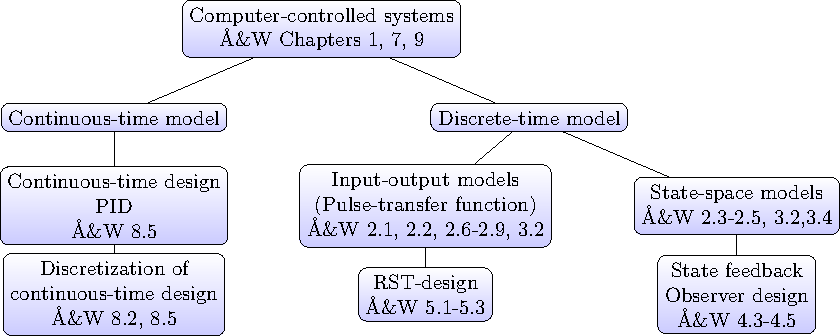
\includegraphics[width=\linewidth]{../figures/computer-control-approaches}
\end{center}
\end{frame}

\begin{frame}[label=sec-4-3]{Discrete time vs continuous time}
\begin{center}
\begin{tabular}{ll}
Continuous time & Discrete time\\
\hline
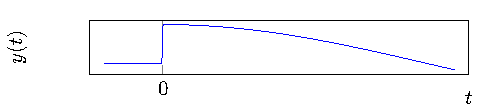
\includegraphics[width=0.4\linewidth]{cont-fcn} & 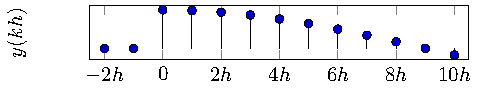
\includegraphics[width=0.4\linewidth]{discrete-fcn}\\
\(y(t)\) & \(y(kh)\)\\
\(\operatorname{p} y \triangleq \frac{d}{dt} y\) & \(\operatorname{q}y \triangleq y(kh+h)\)\\
\( (\operatorname{p}+a) y = bu \;\Leftrightarrow\; \frac{d}{dt}y + ay = bu\) & \( (\operatorname{q} + \alpha) y = \beta u \; \Leftrightarrow \; y(k+1) + \alpha y(k) = \beta u(k)\)\\
\(Y(s) \triangleq \laplace{y(t)}\) & \(Y(z) \triangleq \ztrf{y(kh)}\)\\
\( Y(s) = G(s)U(s) = \frac{b}{s+a}U(s)\) & \(Y(z) = H(z)U(z) = \frac{\beta}{z+\alpha}U(z)\)\\
Pole of the system: \(s+a=0 \; \Rightarrow \; s = -a\) & Pole of the system: \( z+\alpha = 0 \; \Rigtharrow \; z = -\alpha \)\\
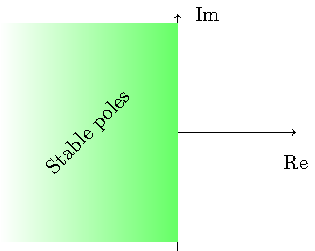
\includegraphics[width=0.22\linewidth]{cont-stable} & 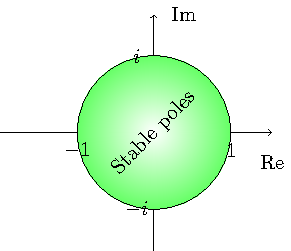
\includegraphics[width=0.22\linewidth]{discrete-stable}\\
\hline
\end{tabular}
\end{center}
\end{frame}

\section{Course structure}
\label{sec-5}
\begin{frame}[label=sec-5-1]{How we will work}
\alert{Prepare, prepare, prepare} for classes:
\begin{enumerate}
\item Read text material and watch video
\item Solve quizz (test) on Blackboard (up to 100p, accounts for 1\% of final grade)
\end{enumerate}
In class:
\begin{enumerate}
\item Review of material
\item Work with concepts
\item Problem solving
\item Summarize
\end{enumerate}
\end{frame}

\begin{frame}[label=sec-5-2]{Course book}
\begin{center}
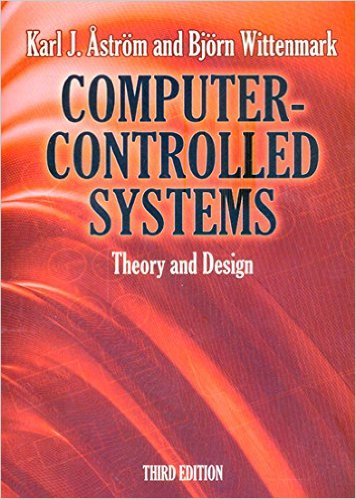
\includegraphics[width=0.2\linewidth]{../figures/book.png}
\end{center}
Buy ebook at Google Books (525 MXN)
\end{frame}

\begin{frame}[label=sec-5-3]{Homework}
\begin{itemize}
\item About every second week
\item Solved individually, handed in on Blackboard
\item Each homework accounts for 4\% of final grade (except first hw which is 2\%)
\end{itemize}
\end{frame}

\begin{frame}[label=sec-5-4]{Project}
\begin{itemize}
\item Implement controller on arduino, accounts for 10\% of final grade
\item Groups of 4 (self-elected)
\item Partial reports (20p)
\item Final report (30p)
\item Demonstrate working open-loop setup (10p)
\item Demonstrate controller design and  working closed-loop system (20p)
\item Individual journal (10p)
\end{itemize}
\end{frame}

\begin{frame}[label=sec-5-5]{Examination}
\begin{itemize}
\item Quizzes 10\%
\item Homework 18\%
\item Project 10\%
\item 2 partial exams (1.5hrs) 36\%
\item Final exam (3hrs) 26\%
\end{itemize}
\end{frame}


\begin{frame}[label=sec-5-6]{Coming up}
\begin{itemize}
\item Homework 1: Repetition of stuff from control engineering. On Bb.
\item See preparation instructions for next week on Bb
\end{itemize}
\end{frame}

\section{Example}
\label{sec-6}
% Emacs 24.5.1 (Org mode 8.2.10)
\end{document}